\documentclass[11pt]{article}
\usepackage[a4paper,margin=2.25cm]{geometry}
\usepackage[T1]{fontenc}
\usepackage[utf8]{inputenc}
\usepackage{lmodern}
\usepackage{amsmath,amssymb,mathtools}
\usepackage{graphicx}
\usepackage{booktabs,tabularx,array}
\usepackage{microtype}
\usepackage{caption}
\usepackage{float}
\usepackage[hidelinks]{hyperref}
\hypersetup{
  pdftitle={Supplementary Material 1 - analytical, numerical and agent-based supplements},
  pdfauthor={Seyfullah Enes Kotil},
  pdfsubject={Analytical details, perturbative construction, agent-based benchmark, and closure validation},
  pdfkeywords={contact tracing, agent-based model, deterministic hierarchy, event-level verification}
}
\usepackage{fancyhdr}
\usepackage{lastpage}
\usepackage{xurl}

\newcommand{\ABM}{\mathrm{ABM}}
\newcommand{\HD}{\mathrm{HD}}
\setlength{\parindent}{0pt}
\setlength{\parskip}{0.58em}
\setlength{\emergencystretch}{3em}
\renewcommand{\arraystretch}{1.12}
\renewcommand{\theequation}{S\arabic{equation}}
\renewcommand{\thefigure}{S\arabic{figure}}
\renewcommand{\thetable}{S\arabic{table}}
\captionsetup[figure]{name=Fig.,font=small,labelfont=bf,labelsep=space,justification=justified,singlelinecheck=false}
\captionsetup[table]{font=small,labelfont=bf,labelsep=space,justification=justified,singlelinecheck=false,position=top}
\pagestyle{fancy}
\fancyhf{}
\fancyhead[L]{\small Supplementary Material 1}
\fancyhead[R]{\small Kotil}
\fancyfoot[C]{\small \thepage\ of \pageref{LastPage}}
\setlength{\headheight}{14pt}
\begin{document}

\pdfbookmark[0]{Supplementary Material 1}{sm1-cover}
\begin{center}
{\Large\bfseries Supplementary Material 1: Supplementary Information}\\[1.0em]
{\large\bfseries Overlapping roots: a transmission-tree framework for population-level contact-tracing dynamics}\\[1.2em]
{\bfseries Journal:} Mathematical Biosciences\\[0.5em]
{\bfseries Author:} Seyfullah Enes Kotil\\[0.4em]
Boğaziçi University, Department of Molecular Biology and Genetics, Istanbul, Türkiye\\
Bahçeşehir University, School of Medicine, Department of Biophysics, Istanbul, Türkiye\\[0.5em]
{\bfseries Corresponding author:} enesseyfullah.kotil@bogazici.edu.tr\\[1.2em]
{\bfseries Supplementary Material 1}\\
Model construction details, analytical and numerical details for the quasi-steady solution, the perturbative construction, technical results and the large-population ensemble protocol, the finite-population agent-based benchmark, closure validation, and reproducibility files
\end{center}
\vspace{0.5em}\hrule\vspace{1em}

\textbf{Associated supplementary files.} Supplementary Material 2 (\texttt{supplementary\_material\_2.xlsx}) contains all 780 dimensional parameterizations, the published trajectory-error and convergence summaries, and deterministic-reference and event-term checks. Supplementary Material 3 (\texttt{supplementary\_material\_3.zip}) contains the available executable and audit code, numerical tables and data, event-term verification data, figure-generation files, and software requirements.

\section*{S1 Model construction details}
\pdfbookmark[1]{S1 Model construction details}{s1}
These derivations underlie Section~2 of the main text.

\subsection*{S1.1 Proportional-allocation benchmark}

The first-generation child-count classes determine the total forward-tracing loss but not the classes from which traced individuals are removed (main-text Section~2.2). A benchmark that closes the system by assumption supposes traced individuals are distributed across the child-count classes in the same proportions as the infectious population as a whole. This is an illustrative closure assumption and is \emph{not} implied by the active-transmission-genealogy construction. Under it, the fraction of tracing-induced removals assigned to class $r$ is $I_r/I$, so for $I>0$
\begin{equation}
\left.\frac{dI_r}{dt}\right|_{\text{forward,prop}} = -\gamma_c p_f M_1 \frac{I_r}{I}.
\end{equation}
Summing over $r$ recovers the total forward-tracing loss $-\gamma_c p_f M_1$, since $\sum_{r\geq0}I_r=I$. Multiplying by $r$ and summing gives the corresponding contribution to $M_1$,
\begin{equation}
\left.\frac{dM_1}{dt}\right|_{\text{forward,prop}} = -\gamma_c p_f M_1 \sum_{r\geq0} r\frac{I_r}{I} = -\gamma_c p_f \frac{M_1^2}{I}.
\end{equation}
Combining with the transmission and primary-removal contributions gives a system closed in $S$, $I$, and $M_1$ alone:
\begin{align}
\frac{dS}{dt} &= -\beta S I, \\
\frac{dI}{dt} &= \beta S I - \Gamma I - \gamma_c p_f M_1, \\
\frac{dM_1}{dt} &= \beta S I - 2\Gamma M_1 - \gamma_c p_f \frac{M_1^2}{I},
\end{align}
where the proportional term is defined for $I>0$ and set to zero at $I=0$, where necessarily $M_1=0$. The population-level loss $-\gamma_c p_f M_1$ follows from the tracing mechanism itself; the term $-\gamma_c p_f M_1^2/I$ does not, and is a consequence of the proportional-allocation assumption. The depth-resolved coordinates of main-text Section~2.3 avoid it.

\subsection*{S1.2 Complete rooted configurations and population classes}

Let $\xi_i(t)$ denote the complete active-descendant configuration associated with root $i$, and $\mathcal X$ the set of possible rooted configurations. For $x\in\mathcal X$, define
\begin{equation}
I_x(t) = \sum_{i\in\mathcal A(t)} \mathbf 1_{\{\xi_i(t)=x\}},
\end{equation}
the number of infectious roots whose rooted views have configuration $x$. The full collection $\{I_x(t)\}_{x\in\mathcal X}$ is a population-level description retaining the complete active genealogical information carried by the rooted views; the first-generation classes $I_r$ are obtained by grouping configurations according to their numbers of active children. If $d_k(x)$ denotes the number of active depth-$k$ descendants in configuration $x$, then
\begin{equation}
M_k(t) = \sum_{x\in\mathcal X} d_k(x) I_x(t),
\end{equation}
which agrees with the definition by summation over rooted views. The depth coordinates $M_k$ therefore arise as aggregates of the complete genealogy-aware classes $I_x$, rather than as independently imposed moment variables. Evolving the complete collection is neither analytically convenient nor necessary for the tracing quantities considered here.

\section*{S2 Analytical and numerical details for the QSS solution}
\pdfbookmark[1]{S2 Analytical and numerical details for the QSS solution}{s2}
This section provides the admissibility argument, numerical evaluation procedure, and stochastic comparison protocol supporting Section~3 of the main text. The notation and main-text equation numbers are retained below.

\subsection*{S2.1 Existence and admissibility of the implicit QSS solution}

For $0<c\leq1$, define
\begin{equation}
F_{R,c}(u)=\sqrt{\frac{R}{c}}\;\frac{I_{R-cu+1}\!\left(2\sqrt{cR}\right)}{I_{R-cu}\!\left(2\sqrt{cR}\right)},
\qquad 0\leq u\leq1.
\label{eq:s2-1}
\end{equation}
The self-consistency condition in main-text Eq.~(3.8) is $F_{R,c}(u)=u$. Since $R-cu>-1$ for $R>0$, $0<c\leq1$, and $0\leq u\leq1$, and since $2\sqrt{cR}>0$, the modified Bessel functions appearing in Eq.~\eqref{eq:s2-1} are positive and continuous. Hence $F_{R,c}$ is continuous and positive on $[0,1]$.

For the positive decaying ratio sequence corresponding to a fixed trial value $u$, main-text Eq.~(3.5) can be written as
\begin{equation}
r_k(u)=\frac{R}{R+k-cu+cr_{k+1}(u)}.
\label{eq:s2-2}
\end{equation}
At $k=1$, $F_{R,c}(u)=r_1(u)$. Therefore,
\begin{equation}
F_{R,c}(1)=\frac{R}{R+1-c+cr_2(1)}<1,
\end{equation}
where the inequality is strict because $r_2(1)>0$. Since $F_{R,c}(0)>0$, the continuous function $F_{R,c}(u)-u$ is positive at $u=0$ and negative at $u=1$. The intermediate value theorem therefore gives at least one self-consistent solution
\begin{equation}
m_1\in(0,1).
\end{equation}
At any such solution, the denominator in Eq.~\eqref{eq:s2-2} exceeds $R$: indeed, $k-cm_1>0$ for every $k\geq1$, and $cr_{k+1}>0$. Hence
\begin{equation}
0<r_k<1,\qquad k\geq1.
\end{equation}
Since $m_k=m_{k-1}r_k$ and $m_0=1$, it follows that
\begin{equation}
1=m_0>m_1>m_2>\cdots>0.
\end{equation}
For $k\geq2$, $cm_1<1$ and $cr_{k+1}>0$, so Eq.~\eqref{eq:s2-2} also gives
\begin{equation}
r_k<\frac{R}{R+k-1}.
\end{equation}
Consequently,
\begin{equation}
0<m_k=m_1\prod_{j=2}^{k}r_j<m_1\prod_{j=2}^{k}\frac{R}{R+j-1}\longrightarrow0\qquad(k\to\infty).
\end{equation}
Thus every positive self-consistent solution of main-text Eq.~(3.8) defines a genealogically admissible descendant sequence.

When $c=0$, main-text Eq.~(3.5) becomes explicit:
\begin{equation}
r_k(R,0)=\frac{R}{R+k},
\qquad
m_k(R,0)=\prod_{j=1}^{k}\frac{R}{R+j},
\label{eq:s2-9}
\end{equation}
and therefore $m_1(R,0)=R/(R+1)$. For each tested $c>0$, the scalar root was obtained independently. Across the tested parameter grid, the selected roots vary continuously from the no-tracing value and thereby identify the positive branch used in main-text Section~3. This selection does not require a claim of global uniqueness for all mathematical roots of main-text Eq.~(3.8).

\subsection*{S2.2 Numerical evaluation of the implicit solution}

The primary calculation solves the scalar residual
\begin{equation}
G_{R,c}(u)=F_{R,c}(u)-u
\end{equation}
for $u\in(0,1)$. At $c=0$, the explicit solution is $u=R/(R+1)$. For each $c>0$, the root was obtained independently by Brent's safeguarded method on $[0,1]$, using absolute and relative tolerances of $10^{-14}$. Across the tested grid, the resulting roots varied continuously from the no-tracing value and remained on the selected positive branch.

Modified-Bessel ratios were evaluated with exponentially scaled functions. Because the numerator and denominator in main-text Eq.~(3.8) have the same argument, the common exponential factor cancels, avoiding overflow or underflow while preserving the required ratio (Amos 1974). For $c>0$, once $m_1$ was obtained, the descendant coordinates were calculated from
\begin{equation}
m_k=\left(\frac{R}{c}\right)^{k/2}\frac{I_{R-cm_1+k}\!\left(2\sqrt{cR}\right)}{I_{R-cm_1}\!\left(2\sqrt{cR}\right)},
\qquad k\geq1.
\end{equation}
At $c=0$, the explicit expression in Eq.~\eqref{eq:s2-9} was used.

As an independent consistency calculation, the continued fraction was evaluated by backward recursion. For a terminal depth $K$, set
\begin{equation}
r_{K+1}^{(K)}=0
\end{equation}
and compute
\begin{equation}
r_k^{(K)}=\frac{R}{R+k-cm_1+cr_{k+1}^{(K)}},
\qquad k=K,K-1,\ldots,1.
\end{equation}
The truncated self-consistency equation $r_1^{(K)}=m_1$ was solved separately at $K=40$ and $K=80$. Over the main-text Fig.~2 grid, the maximum fixed-point residual of the scaled-Bessel calculation was below $3\times10^{-15}$; the largest difference between the $K=40$ and $K=80$ values of $m_1$, $m_2$, and $m_3$ was below $10^{-15}$, and the largest difference between the scaled-Bessel and $K=80$ continued-fraction calculations was below $10^{-15}$. The verification script and cellwise numerical results are supplied in Supplementary Material~3.

\subsection*{S2.3 Constant-pool stochastic comparison protocol}

The constant-pool simulations use
\begin{equation}
R\in\{1,1.5,2,4\},\qquad c\in\{0,0.25,0.5,0.75,1\},
\end{equation}
with dimensionless rates
\begin{equation}
\Gamma=1,\qquad \gamma=0,\qquad \gamma_c=1,\qquad p_f=c.
\end{equation}
The susceptible pool is held constant, so transmission occurs at total rate $RI$. Tracing is active from $\tau=0$. Each realization begins with 160 unrelated infectious roots, and 120 independent realizations are generated for every parameter pair over $0\leq\tau\leq3.25$.

For each active realization, the normalized descendant coordinate is
\begin{equation}
m_k(\tau)=\frac{M_k(\tau)}{I(\tau)},\qquad I(\tau)>0.
\end{equation}
A coordinate is left undefined after the realization no longer has an active infectious population; no stopped or terminal genealogy is carried forward.

The normalized coordinates were evaluated on the uniform output grid used to generate main-text Fig.~2. Because the output spacing is uniform, equal weighting of the retained observations gives the corresponding discrete time average. For replicate $\ell$ and depth $k$, let $\mathcal T_{k,\ell}$ be the recorded times in the prespecified interval
\begin{equation}
3\leq\tau\leq3.25
\end{equation}
for which $I(\tau)>0$ and $m_k(\tau)$ is defined. The replicate-level summary is
\begin{equation}
m_{k,\ell}^{\ABM}=\frac{1}{|\mathcal T_{k,\ell}|}\sum_{\tau_j\in\mathcal T_{k,\ell}}m_k(\tau_j),
\end{equation}
provided $|\mathcal T_{k,\ell}|>0$. Thus, values after extinction are never imputed or carried forward; a replicate is excluded for depth $k$ only when it has no defined observation in the averaging interval.

Let $\mathcal V_k$ denote the replicates with a defined summary and $n_k=|\mathcal V_k|$. The signed difference plotted in Fig.~2a--c is
\begin{equation}
e^{\ABM}_{k,\mathrm{QSS}}=\frac{1}{n_k}\sum_{\ell\in\mathcal V_k}m_{k,\ell}^{\ABM}-m_k^{\mathrm{QSS}},
\qquad k=1,2,3.
\end{equation}
Percentile 95\% confidence intervals were obtained from 2,000 bootstrap resamples of complete replicate-level summaries; recorded time points within a realization were therefore never resampled as independent observations. For the trajectory panels, complete replicate trajectories were resampled and the ensemble mean was recalculated at each recorded time to obtain pointwise 95\% confidence intervals. The representative panels use $R=2$ and $c=1$; the pale-yellow region marks the averaging interval and the horizontal dashed line gives the selected QSS target.

\section*{S3 Perturbative construction of the QSS approximation}
\pdfbookmark[1]{S3 Perturbative construction of the QSS approximation}{s3}
This section derives the explicit low-order approximation to $m_1$ quoted in
Section~3.2 of the main text, and reports its accuracy against the selected
QSS branch.

\subsection*{S3.1 Rescaled QSS recurrence}

At $c=0$, the QSS recurrence has the no-tracing solution
\begin{equation}
m_{k,0}=\prod_{j=1}^{k}\frac{R}{R+j},
\qquad k\geq1.
\end{equation}
Define
\begin{equation}
\widehat m_k=\frac{m_k}{m_{k,0}},
\qquad
b_k=\frac{R+1}{R+k},
\qquad
\chi_k=\frac{R+1}{R+k+1},
\qquad
\varepsilon=\frac{cR}{(R+1)^2}.
\end{equation}
Substitution into the QSS recurrence gives
\begin{equation}
\widehat m_k=\widehat m_{k-1}+\varepsilon b_k\left(\widehat m_1\widehat m_k-\chi_k\widehat m_{k+1}\right),
\qquad k\geq1.
\label{eq:s3-2}
\end{equation}
For $R>0$ and $0\leq c\leq1$,
\begin{equation}
0\leq\varepsilon\leq\frac{R}{(R+1)^2}\leq\frac14.
\end{equation}
The final inequality follows from $(R-1)^2\geq0$ and is sharp at $R=1$, $c=1$.

\subsection*{S3.2 Coefficient recursion and finite genealogical dependence}

Use the regular expansion
\begin{equation}
\widehat m_k=1+\sum_{n\geq1}a_{k,n}\varepsilon^n,
\qquad a_{k,0}=1,
\qquad a_{0,n}=0\;\;(n\geq1).
\end{equation}
Matching equal powers of $\varepsilon$ in Eq.~\eqref{eq:s3-2} yields
\begin{equation}
a_{k,n}=a_{k-1,n}+b_k\left[\sum_{j=0}^{n-1}a_{1,j}a_{k,n-1-j}-\chi_ka_{k+1,n-1}\right],
\qquad n\geq1.
\label{eq:s3-5}
\end{equation}
The recursion couples adjacent descendant depths while lowering the perturbative order by one in the deeper term. Consequently,
\[
a_{1,p}\longrightarrow a_{2,p-1}\longrightarrow\cdots\longrightarrow a_{p,1}\longrightarrow a_{p+1,0}.
\]
The deepest required quantity is the known no-tracing coefficient $a_{p+1,0}=1$. Hence every fixed perturbative order is determined by a finite genealogical calculation.

For $k=1$,
\begin{align}
a_{1,1}&=\frac{1}{R+2},\\
a_{1,2}&=\frac{7+2R-R^2}{(R+2)^2(R+3)}.
\end{align}
Therefore,
\begin{equation}
m_1^{[p]}(R,c)=\frac{R}{R+1}\left[1+\sum_{n=1}^{p}a_{1,n}(R)\left(\frac{cR}{(R+1)^2}\right)^n\right].
\end{equation}
The formulas used in Fig.~\ref{fig:S7-1} are
\begin{align}
m_1^{[0]}&=\frac{R}{R+1},\\
m_1^{[1]}&=\frac{R}{R+1}\left[1+\frac{cR}{(R+1)^2(R+2)}\right],\\
m_1^{[2]}&=\frac{R}{R+1}\left[1+\frac{cR}{(R+1)^2(R+2)}+\frac{7+2R-R^2}{(R+2)^2(R+3)}\left(\frac{cR}{(R+1)^2}\right)^2\right].
\end{align}

\subsection*{S3.3 Local finite-depth basis}

Consider a finite truncation retaining $\widehat m_1,\ldots,\widehat m_K$ and an analytic terminal prescription $\widehat m_{K+1}=T_K(\varepsilon)$ satisfying $T_K(0)=1$. The truncated QSS equations are analytic in the retained moments and $\varepsilon$. At $\varepsilon=0$, Eq.~\eqref{eq:s3-2} reduces to $\widehat m_k=\widehat m_{k-1}$, so the no-tracing solution is $\widehat m_k=1$. The Jacobian with respect to the retained moments is lower bidiagonal with unit diagonal and is therefore nonsingular. Standard analytic implicit-function and regular-perturbation arguments consequently give a locally unique analytic branch whose coefficients satisfy Eq.~\eqref{eq:s3-5} (Krantz and Parks 2002; Murdock 1999).

This is a local statement for each fixed finite truncation. The main-text claim does not require a global convergence theorem for the complete infinite series; instead, the accuracy of the explicit low-order formulas is assessed directly against the selected QSS branch.

\subsection*{S3.4 Numerical evaluation for the perturbative accuracy figure}

The selected QSS branch was evaluated by solving the scalar fixed-point equation generated by a backward continued fraction. Fig.~\ref{fig:S7-1} was generated using continued-fraction depth 80 and a bracketed scalar solve on $0\leq m_1\leq1$. The error curves were evaluated at $R\in\{1,1.5,2,4\}$ and at 1001 equally spaced values of $c$ on $[0,1]$. For retained order $p$,
\begin{equation}
e_p^{\mathrm{pert}}(R,c)=\left|m_1^{[p]}(R,c)-m_1^{\mathrm{QSS}}(R,c)\right|.
\end{equation}
The maximum errors over the $c$-grid are summarized in Table~\ref{tab:S7-1}.

\begin{table}[H]
\centering
\caption{Maximum absolute perturbative errors $e_p^{\mathrm{pert}}$ over $c\in[0,1]$ for the parameter values used in Fig.~\ref{fig:S7-1}.}
\label{tab:S7-1}
\small
\begin{tabular}{@{}rccc@{}}
\toprule
$R$ & $p=0$ & $p=1$ & $p=2$ \\
\midrule
1.0 & $5.0374326\times10^{-2}$ & $8.7076597\times10^{-3}$ & $1.7632153\times10^{-3}$ \\
1.5 & $4.6553438\times10^{-2}$ & $5.4105804\times10^{-3}$ & $5.5180492\times10^{-4}$ \\
2.0 & $3.9907541\times10^{-2}$ & $2.8705039\times10^{-3}$ & $1.0154532\times10^{-5}$ \\
4.0 & $2.1111821\times10^{-2}$ & $2.2151187\times10^{-4}$ & $1.4024202\times10^{-4}$ \\
\bottomrule
\end{tabular}
\end{table}

For every displayed $R$ and $p$, the maximum occurred at $c=1$. The signed $p=2$ error for $R=2$ crossed zero at $c=0.8942672386$.

\begin{figure}[H]
\centering
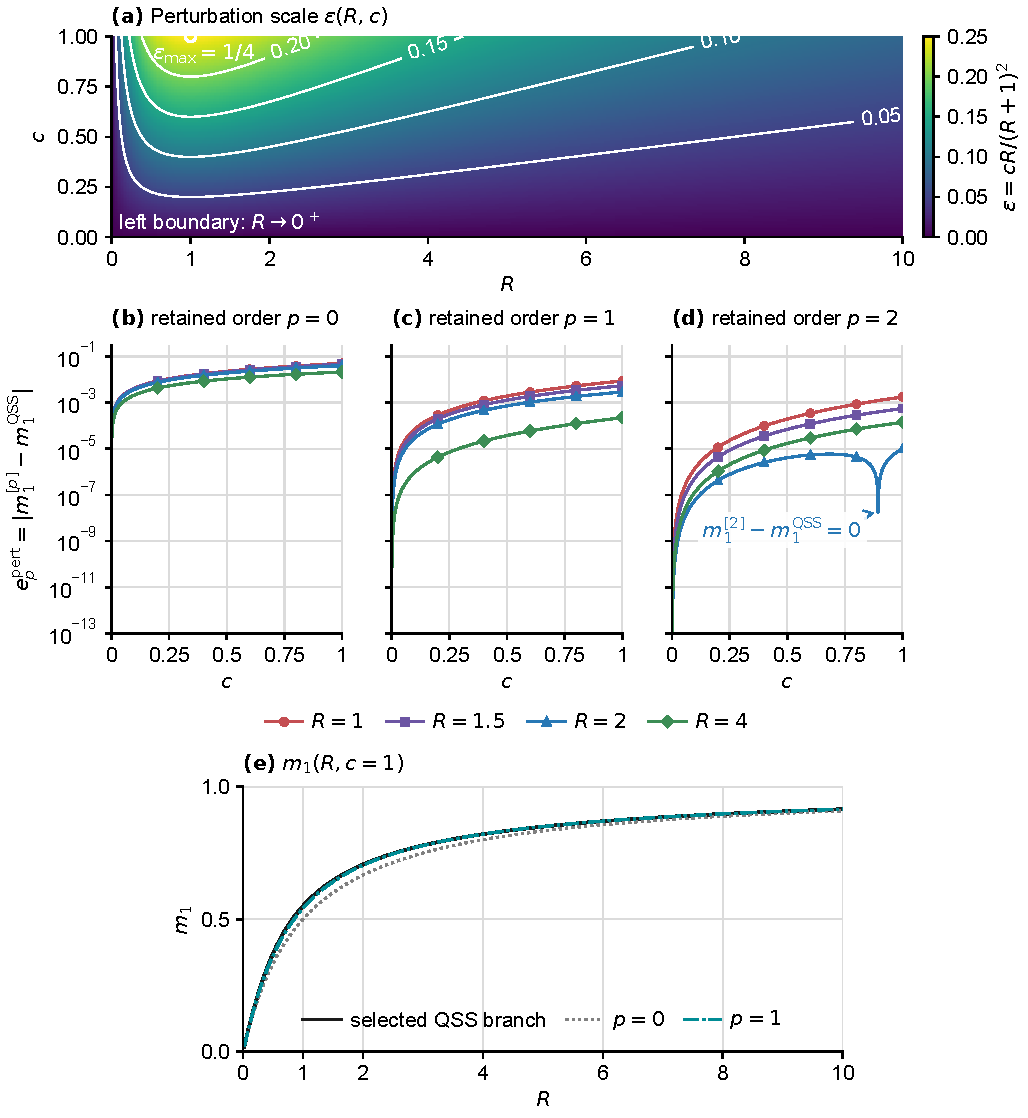
\includegraphics[width=0.92\textwidth]{figures/supp_S7_perturbation_accuracy.pdf}
\caption{Effective perturbation scale and numerical accuracy of the explicit QSS approximation. (a) The perturbation scale $\varepsilon=cR/(R+1)^2$ over $0<R\leq10$ and $0\leq c\leq1$. It satisfies $0\leq\varepsilon\leq1/4$, with equality at $R=1$ and $c=1$; the displayed left boundary represents the limit $R\to0^+$. (b--d) Absolute errors $e_p^{\mathrm{pert}}=|m_1^{[p]}-m_1^{\mathrm{QSS}}|$ for retained orders $p=0,1,2$, respectively, at $R=1,1.5,2$, and $4$. Errors vanish at $c=0$ and are omitted from the logarithmic axes. The narrow minimum in the $R=2$ curve in panel (d) occurs where the signed second-order error crosses zero near $c=0.894$. (e) The selected QSS branch and the $p=0$ and $p=1$ approximations along $c=1$. The first-order approximation is already nearly coincident with the selected branch over the displayed range. These errors compare the explicit perturbative formulas against the selected QSS branch itself; they are not errors of the QSS branch relative to the underlying epidemic process, which is assessed separately in main-text Section~3.3.}
\label{fig:S7-1}
\end{figure}

The QSS solver was checked over $R\in[0.05,10]$ and $c\in[0.01,1]$ on a $124\times100$ diagnostic grid. Depths 40, 80, and 160 agreed to double-precision resolution. At depth 160, the maximum fixed-point residual was $2.33\times10^{-15}$, and the maximum discrepancy between the continued-fraction evaluation and the evaluation based on the modified-Bessel representation was $4.44\times10^{-15}$.

\section*{S4 Technical results and large-population ABM ensemble protocol}
\pdfbookmark[1]{S4 Technical results and large-population ABM ensemble protocol}{s4}
These technical results and the ensemble protocol support the epidemiological
observables and the control boundary of Section~4 of the main text.

\subsection*{S4.1 Equality of the growth and replacement thresholds}

On the selected constant-pool QSS branch, the normalized moments satisfy
\begin{equation}
0=R(m_{k-1}-m_k)-km_k+c(m_1m_k-m_{k+1}),
\qquad k\geq1,
\label{eq:S8-qss-recurrence}
\end{equation}
with $m_0=1$. Define
\begin{equation}
B(R,c)=1+\sum_{k\geq1}\frac{(-c)^k}{(k+1)!}\,m_k(R,c).
\label{eq:S8-B-definition}
\end{equation}
The factorial weights make all sums below absolutely convergent. Multiply Eq.~\eqref{eq:S8-qss-recurrence} by $(-c)^k/(k+1)!$ and sum over $k\geq1$. After index shifts, the transmission terms generate the series in $\mathcal R_{\mathrm{time}}$, while the remaining terms collect into $gB$, giving
\begin{equation}
\mathcal R_{\mathrm{time}}(R,c)-1
=g(R,c)B(R,c).
\label{eq:S8-threshold-identity}
\end{equation}
For completeness, the weighted sum can be written directly as
\begin{align}
0
&=\sum_{k\geq1}\frac{(-c)^k}{(k+1)!}
\left[R(m_{k-1}-m_k)-km_k+c(m_1m_k-m_{k+1})\right] \\
&=\mathcal R_{\mathrm{time}}-1-gB.
\label{eq:S8-weighted-sum}
\end{align}
Moreover, Eq.~\eqref{eq:S8-B-definition} is an alternating series with strictly decreasing term magnitudes because
\begin{equation}
\frac{c^{k+1}m_{k+1}/(k+2)!}{c^km_k/(k+1)!}
=\frac{c}{k+2}\frac{m_{k+1}}{m_k}
\leq\frac{1}{k+2}<1.
\end{equation}
Hence
\begin{equation}
B(R,c)\geq1-\frac{cm_1}{2}>\frac12.
\label{eq:S8-B-positive}
\end{equation}
Therefore
\begin{equation}
g(R,c)=0
\quad\Longleftrightarrow\quad
\mathcal R_{\mathrm{time}}(R,c)=1,
\label{eq:S8-threshold-equivalence}
\end{equation}
although the two quantities have different numerical values and interpretations away from the boundary.

\subsection*{S4.2 Finite-depth evaluation of $\mathcal R_{\mathrm{time}}$}

Retaining genealogical coordinates through $m_{K-1}$, define
\begin{equation}
\mathcal R_{\mathrm{time}}^{(K)}(R,c)
=R\left[
1+\sum_{k=0}^{K-1}\frac{(-c)^{k+1}}{(k+2)!}\,m_k(R,c)
\right].
\label{eq:S8-Rtime-K}
\end{equation}
Because $m_k$ is nonincreasing and $0\leq c\leq1$, the omitted tail is alternating with decreasing magnitude. Its error is bounded by the first omitted term:
\begin{equation}
\left|
\mathcal R_{\mathrm{time}}-
\mathcal R_{\mathrm{time}}^{(K)}
\right|
\leq
R\frac{c^{K+1}}{(K+2)!}\,m_K
\leq Rm_K.
\label{eq:S8-Rtime-tail}
\end{equation}
The factorial factor makes the lifetime replacement quantity substantially less sensitive to deep-tail error than an unweighted moment sum.

\subsection*{S4.3 Propagation of QSS approximation errors}

If an approximation $m_1^{[p]}$ is used in the growth rate, then
\begin{equation}
g^{[p]}-g^{\mathrm{QSS}}
=-c\left(m_1^{[p]}-m_1^{\mathrm{QSS}}\right).
\label{eq:S8-growth-error}
\end{equation}
If approximate moments $m_k^{[p]}$ are used through depth $K-1$, then
\begin{align}
\left|
\mathcal R_{\mathrm{time}}^{[p,K]}
-
\mathcal R_{\mathrm{time}}^{\mathrm{QSS}}
\right|
&\leq
R\sum_{k=1}^{K-1}
\frac{c^{k+1}}{(k+2)!}
\left|m_k^{[p]}-m_k^{\mathrm{QSS}}\right| \\
&\quad+
R\frac{c^{K+1}}{(K+2)!}m_K^{\mathrm{QSS}}.
\label{eq:S8-Rtime-error}
\end{align}
The first term is the error in the retained coordinates and the second is the unresolved genealogical tail. This analysis concerns approximation of the selected QSS branch; it is distinct from finite-population ABM--QSS discrepancy.

\subsection*{S4.4 Large-population constant-pool ABM ensemble protocol}

The ABM uses the same transmission, primary-removal, detection, and instantaneous one-step forward-tracing events as the deterministic hierarchy. The susceptible pool is held constant in the transmission rate. The decomposition used for main-text Fig.~3 is
\begin{equation}
\frac{\gamma}{\Gamma}=0,
\qquad
\frac{\gamma_c}{\Gamma}=1,
\qquad
p_f=c.
\label{eq:S8-abm-decomposition}
\end{equation}
Thus, the deterministic prediction depends on $R$ and $c$, while the ABM realizes the corresponding finite-population event system.

\begin{table}[H]
\centering
\caption{Simulation design used for main-text Fig.~3.}
\label{tab:S8-simulation-design}
\scriptsize
\begin{tabular}{p{0.18\textwidth}p{0.29\textwidth}p{0.43\textwidth}}
\toprule
Component & Cells & Design \\
\midrule
Panels (a)--(b) & $R=1,1.5,2,4$; $c=0,0.25,0.5,0.75,1$ & 300 independent paths per cell; prespecified burn-in and windows; whole-replicate bootstrap intervals. \\
Cohort follow-up & Same 20 cells & Complete follow-up of every entrant; no lifetime or required production interval is censored. \\
Panel (c) & $c=0.25,0.5,0.75,1$; two prespecified $R$-bracketing cells & Pooled growth estimates, linear interpolation, and pointwise whole-replicate bootstrap intervals. \\
\bottomrule
\end{tabular}
\end{table}

For replicate $r$, let
\begin{equation}
P_r=\int_{\tau_{0,r}}^{\tau_{1,r}}I_r(\tau)\,d\tau
\label{eq:S8-parent-person-time}
\end{equation}
be the parent infectious person-time in the prespecified measurement or cohort-entry window. If $N_{+,r}$ is the number of new infections and $N_{-,r}$ is the number of infectious individuals removed by primary removal or tracing during the growth-measurement window, the pooled event/person-time estimator is
\begin{equation}
\widehat g
=
\frac{\sum_r(N_{+,r}-N_{-,r})}{\sum_rP_r}.
\label{eq:S8-g-estimator}
\end{equation}
Here $N_{-,r}$ counts removed individuals rather than removal-event occurrences, so tracing events that remove more than one infectious individual contribute their full population change.

Let $\mathcal C_r$ be the set of infections entering during the cohort window, and let $L_{jr}$ be the complete remaining infectious lifetime of cohort member $j$. The pooled infectious-time replacement estimator is
\begin{equation}
\widehat{\mathcal R}_{\mathrm{time}}
=
\frac{\displaystyle\sum_r\sum_{j\in\mathcal C_r}L_{jr}}
{\displaystyle\sum_rP_r}.
\label{eq:S8-Rtime-estimator}
\end{equation}
The event system is continued along each path until every enrolled cohort member has been removed. The entry window, burn-in rule, and production sample size are fixed before the confirmatory runs.

Confidence intervals are obtained by resampling complete replicates and recomputing the pooled ratio in Eqs.~\eqref{eq:S8-g-estimator} and~\eqref{eq:S8-Rtime-estimator}. Serial observations within a replicate are not treated as independent. For panel (c), let $(R^-,\widehat g^-)$ and $(R^+,\widehat g^+)$ denote the two prespecified cells bracketing zero. The interpolated estimate is
\begin{equation}
\widehat R_*(c)
=R^-+
\frac{-\widehat g^-}{\widehat g^+-\widehat g^-}
(R^+-R^-),
\label{eq:S8-threshold-estimator}
\end{equation}
and each bootstrap resample recomputes the two pooled growth estimates and the interpolation.

\subsection*{S4.5 Analytical and numerical checks}

The analytical curves use the same selected-QSS solver as Fig.~\ref{fig:S7-1} and main-text Fig.~3. The final audit gave a maximum fixed-point residual of $1.887\times10^{-13}$, a maximum accepted depth-doubling difference of $1.943\times10^{-13}$, and a maximum modified-Bessel/continued-fraction difference of $1.894\times10^{-13}$. The control-boundary values used in Fig.~4c are
\begin{equation}
\begin{array}{c|ccccc}
c & 0 & 0.25 & 0.50 & 0.75 & 1.00\\ \hline
R_*(c) & 1.00000000 & 1.13568648 & 1.29328143 & 1.47215210 & 1.66978036
\end{array}.
\label{eq:S8-critical-values}
\end{equation}
The threshold identity was checked on 8,888 parameter points. Across the 20 cohort cells, the maximum relative Monte Carlo standard error was 0.50\%, the maximum analytical discrepancy was 0.67\%, and 19 of 20 pointwise intervals contained their targets; all panel-(c) intervals contained the analytical critical curve. These comparisons assess large-population ensemble behavior of the same event system, not an unrelated stochastic model.

\section*{S5 Finite-population agent-based benchmark}
\pdfbookmark[1]{S5 Finite-population agent-based benchmark}{s5}
This section documents the individual-level benchmark introduced in
Section~2.4 of the main text and used for the comparisons reported in
Sections~3.3, 4.2 and 5.2.

\subsection*{S5.1 The agent-based model}
The finite-population agent-based model (ABM) simulates transmission, spontaneous removal, detection, and instantaneous one-step forward tracing on the active transmission forest. Individual identities and unique infector--infectee links are retained throughout each realization. Let $U^{\mathrm{ABM}}(t)$ and $I^{\mathrm{ABM}}(t)$ denote the susceptible and infectious counts in physical time. Transmission, spontaneous removal, and detection occur at total rates
\[
\beta U^{\mathrm{ABM}}(t)I^{\mathrm{ABM}}(t),\qquad
\gamma I^{\mathrm{ABM}}(t),\qquad
\gamma_c I^{\mathrm{ABM}}(t),
\]
respectively. At transmission, an infectious individual is selected uniformly as the infector, one susceptible individual becomes infectious, and the new case is recorded as an active child of its infector. At spontaneous removal, the selected individual leaves the active infectious set. At detection, the selected individual is removed and each active direct infectee is independently removed with probability $p_f$; traced removals do not initiate further tracing. Descendant-depth observables $M_k^{\mathrm{ABM}}(t)$ can be computed directly from the active transmission forest at each observation time; the numerical trajectory comparison uses $M_1^{\mathrm{ABM}}$. The process is simulated with an exact event-driven Gillespie algorithm.

The dimensional parameters determine
\[
\Gamma=\gamma+\gamma_c,\qquad
\tau=\Gamma t,\qquad
R=\frac{\beta U_0}{\Gamma},\qquad
c=\frac{\gamma_c p_f}{\Gamma}.
\]
The process is simulated in physical time and reported on $0\leq\tau\leq5$. Detection operates throughout the comparison experiments, whereas forward tracing is activated at $\tau_{\mathrm{on}}=0.5$. The same activation schedule is imposed in the deterministic reference.

\subsection*{S5.2 Crossed dimensional parameterizations}
The nondimensional parameters $R$ and $c$ do not uniquely determine the dimensional rates. We therefore cross
\[
\Gamma\in\left\{\frac14,\frac12,1,2,4\right\}
\]
with three explicit detection--tracing decompositions. For prescribed $R$, $c$, $U_0$, and $\Gamma$, the parameterizations are
\begin{table}[H]
\caption{Crossed dimensional parameterizations for $0\leq c<1$}
\centering\small
\begin{tabularx}{\textwidth}{@{}p{0.34\textwidth}cccc@{}}
\toprule
Decomposition & $\beta$ & $\gamma$ & $\gamma_c$ & $p_f$ \\
\midrule
Less-frequent detection, complete tracing & $R\Gamma/U_0$ & $\Gamma(1-c)$ & $\Gamma c$ & $1$ \\
Intermediate & $R\Gamma/U_0$ & $\Gamma(1-c)/2$ & $\Gamma(1+c)/2$ & $2c/(1+c)$ \\
Frequent detection, partial tracing & $R\Gamma/U_0$ & $0$ & $\Gamma$ & $c$ \\
\bottomrule
\end{tabularx}
\end{table}
Every row satisfies
\[
\gamma+\gamma_c=\Gamma,\qquad
\frac{\beta U_0}{\Gamma}=R,\qquad
\frac{\gamma_c p_f}{\Gamma}=c.
\]
At $c=1$, the three rows coincide, and one parameterization is retained for each value of $\Gamma$. At $c=0$, the three rows differ in the labeling of primary removal, but no tracing removal occurs.

The analysis uses $R\in\{2,4,6\}$ and $c\in\{0,0.25,0.5,0.75,1\}$. For each population scale, this gives 195 raw-rate protocols: 65 for each value of $R$. All raw-rate protocols are simulated directly. For $U_0\in\{500,1000,2000\}$, one independent pool of 120 trajectories is generated per protocol for population-size convergence. At $U_0=8000$, 30 independent pools of 120 trajectories are generated for every protocol; the first prespecified pool (pool 0) is also used as the $U_0=8000$ point in the population-size comparison. The 30 pools give
\[
195\times30\times120=702{,}000
\]
ABM trajectories at the selected population scale.

\begin{table}[H]
\caption{Global numerical settings}
\centering\small
\begin{tabularx}{\textwidth}{@{}p{0.34\textwidth}X@{}}
\toprule
Setting & Value \\
\midrule
Nondimensional grid & $R\in\{2,4,6\}$, $c\in\{0,0.25,0.5,0.75,1\}$ \\
Dimensional rate scales & $\Gamma\in\{1/4,1/2,1,2,4\}$ \\
Population scales & $U_0\in\{500,1000,2000,8000\}$, $I_0=0.02U_0$ \\
Raw-rate protocols & 195 per population scale; 780 parameterizations in total \\
Population convergence & One 120-realization pool per protocol; at $U_0=8000$, pool 0 of the 30 replicate-convergence pools is used \\
Replicate convergence at $U_0=8000$ & 30 independent 120-realization pools per raw-rate protocol \\
Observation grid & 151 equally spaced points on $0\leq\tau\leq5$ \\
Tracing activation & $\tau_{\mathrm{on}}=0.5$ \\
High-depth reference & $K_{\mathrm{ref}}=40$, checked against $K=80$ \\
Deterministic solver & BDF; relative tolerance $10^{-10}$, absolute tolerance $10^{-12}$, maximum step $0.025$ \\
Pointwise confidence intervals & Normal approximation; conditional on $I(\tau)>0$ for $m_1$ \\
Master seed & 20260804 \\
\bottomrule
\end{tabularx}
\end{table}

\subsection*{S5.3 High-depth deterministic reference}
For each $(R,c)$, the ABM ensemble mean is compared with a high-depth numerical solution retaining $U$, $I$, and $M_1,\ldots,M_{K_{\mathrm{ref}}}$, with $K_{\mathrm{ref}}=40$. The initial state is
\[
U(0)=U_0,\qquad I(0)=I_0,\qquad M_k(0)=0\quad(k\geq1).
\]
At the terminal retained level, $M_{K_{\mathrm{ref}}+1}=0$ is imposed. High-depth trajectories are computed with the BDF method using relative tolerance $10^{-10}$, absolute tolerance $10^{-12}$, and maximum dimensionless step size $0.025$. The intervals before and after $\tau_{\mathrm{on}}=0.5$ are integrated separately so that the change in the tracing terms is imposed exactly at the activation time. The structural bound $0\leq M_{K_{\mathrm{ref}}+1}\leq M_{K_{\mathrm{ref}}}$ follows from Lemma 1 of the main manuscript, but adequacy is assessed independently by repeating the calculation with $K=80$. Across the full grid and observation interval, the maximum absolute difference in $(U/U_0,I/U_0,M_1/U_0)$ was $2.99\times10^{-10}$.

\subsection*{S5.4 Ensemble-mean trajectory error and convergence}
For realization $\ell$, define
\[
\mathbf z^{\mathrm{ABM},(\ell)}(\tau)=\left(\frac{U^{\mathrm{ABM},(\ell)}}{U_0},\frac{I^{\mathrm{ABM},(\ell)}}{U_0},\frac{M_1^{\mathrm{ABM},(\ell)}}{U_0}\right).
\]
For a pool of $n$ independent realizations, $\overline{\mathbf z}_n^{\mathrm{ABM}}=n^{-1}\sum_{\ell=1}^n\mathbf z^{\mathrm{ABM},(\ell)}$. With $\mathbf z^{\mathrm{HD}}$ denoting the high-depth trajectory,
\[
E_{\mathrm{mean}}=\left[\frac1T\int_0^T\left\|\overline{\mathbf z}_n^{\mathrm{ABM}}(\tau)-\mathbf z^{\mathrm{HD}}(\tau)\right\|_2^2\,\mathrm d\tau\right]^{1/2}.
\]
The integral is evaluated over $0\leq\tau\leq5$ at 151 equally spaced observation times using the trapezoidal rule. Extinct realizations remain at $I^{\mathrm{ABM}}=M_1^{\mathrm{ABM}}=0$ and contribute to unconditional scaled-count means. Pointwise 95\% confidence intervals in Figs.~\ref{fig:s2} and~\ref{fig:s3} are calculated as $\overline{x}(\tau)\pm1.96s_x(\tau)/\sqrt{n_\tau}$. For $U$, $I$, and $M_1$, $n_\tau=120$. For $m_1=M_1/I$, the mean, standard deviation, and confidence interval are calculated conditionally over realizations satisfying $I(\tau)>0$, and $n_\tau$ is the number of contributing nonextinct realizations.

For population-size convergence, one 120-realization pool is used for each raw-rate protocol. For $U_0\in\{500,1000,2000\}$, this pool is generated independently for the population-size calculation. At $U_0=8000$, the first prespecified pool (pool 0) among the 30 pools generated for replicate convergence is reused in the population-size comparison. For replicate convergence at $U_0=8000$, every raw-rate protocol has 30 independent master pools. Within each pool, the 120 trajectories are randomly permuted once, and the first $n$ trajectories are used for $n\in\{1,2,5,10,20,40,80,120\}$. Thus, each value of $n$, including $n=120$, has
\[
195\times30=5850
\]
independent ensemble-error estimates. Estimates at different values of $n$ are paired within a pool, but the 5850 estimates at any fixed $n$ arise from independent pools. The representative trajectory plots in Figs.~\ref{fig:s2}--\ref{fig:s4} use the first prespecified independently generated pool (pool 0) for each displayed protocol; no pool was selected according to its agreement with the deterministic reference.

\begin{table}[H]
\caption{Population-size convergence. Each row summarizes one 120-realization ensemble for each of the 195 raw-rate protocols. For $U_0=8000$, the first prespecified pool (pool 0) among the 30 independently generated pools is used.}
\centering\footnotesize
\begin{tabular}{@{}rrrrrrr@{}}
\toprule
$U_0$ & $I_0$ & Protocols & Estimates & Median & 10th percentile & 90th percentile \\
\midrule
500 & 10 & 195 & 195 & 0.012926 & 0.006713 & 0.026509 \\
1000 & 20 & 195 & 195 & 0.006759 & 0.002899 & 0.013034 \\
2000 & 40 & 195 & 195 & 0.003335 & 0.001572 & 0.006732 \\
8000 & 160 & 195 & 195 & 0.001337 & 0.000664 & 0.002717 \\
\bottomrule
\end{tabular}
\end{table}

\begin{table}[H]
\caption{Replicate convergence at $U_0=8000$. Thirty independent 120-realization pools were generated for each of the 195 raw-rate protocols. Consequently, every value of $n$, including $n=120$, is summarized by 5850 independent ensemble-error estimates.}
\centering\footnotesize
\begin{tabular}{@{}rrrrrrr@{}}
\toprule
$n$ & Protocols & Pools/protocol & Estimates & Median & 10th percentile & 90th percentile \\
\midrule
1 & 195 & 30 & 5850 & 0.012499 & 0.006548 & 0.027396 \\
2 & 195 & 30 & 5850 & 0.008872 & 0.004631 & 0.019258 \\
5 & 195 & 30 & 5850 & 0.005733 & 0.002934 & 0.012062 \\
10 & 195 & 30 & 5850 & 0.003970 & 0.002051 & 0.008892 \\
20 & 195 & 30 & 5850 & 0.002852 & 0.001492 & 0.006218 \\
40 & 195 & 30 & 5850 & 0.002062 & 0.001051 & 0.004493 \\
80 & 195 & 30 & 5850 & 0.001532 & 0.000775 & 0.003413 \\
120 & 195 & 30 & 5850 & 0.001308 & 0.000654 & 0.002885 \\
\bottomrule
\end{tabular}
\end{table}

\subsection*{S5.5 Supplementary numerical results}
Population-size convergence was systematic: increasing $U_0$ from 500 to 8000 reduced the median ensemble-mean trajectory error from 0.012926 to 0.001337, with a descriptive log--log slope of -0.82 over the tested population scales. On this basis, $U_0=8000$ was selected as the finite-population benchmark. It was the largest population examined, yielded discrepancies of order $10^{-3}$, and remained computationally feasible for the full crossed parameter design. This is an empirically supported working scale rather than a universal threshold, and the reported discrepancies are empirical summaries rather than rigorous error bounds.

At $U_0=8000$, $I_0=160$, and $n=120$, the 5850 independently generated ensembles had median trajectory error 0.001308, mean 0.001578, 90th percentile 0.002885, and maximum 0.006918. The descriptive log--log slope with replicate count was -0.48, close to the $n^{-1/2}$ reference scaling.

\begin{table}[H]
\caption{Trajectory-error summary by nondimensional grid cell at $U_0=8000$ and $n=120$. Each raw-rate protocol contributes 30 independently generated ensembles.}
\centering\scriptsize
\begin{tabular}{@{}rrrrrrrr@{}}
\toprule
$R$ & $c$ & Protocols & Estimates & Median & Mean & 90th percentile & Maximum \\
\midrule
2 & 0 & 15 & 450 & 0.001786 & 0.002104 & 0.003983 & 0.006454 \\
2 & 0.25 & 15 & 450 & 0.002028 & 0.002302 & 0.004118 & 0.006816 \\
2 & 0.5 & 15 & 450 & 0.001761 & 0.002100 & 0.003910 & 0.006918 \\
2 & 0.75 & 15 & 450 & 0.001658 & 0.001950 & 0.003545 & 0.006671 \\
2 & 1 & 5 & 150 & 0.001613 & 0.001772 & 0.003014 & 0.005445 \\
4 & 0 & 15 & 450 & 0.001225 & 0.001402 & 0.002466 & 0.004225 \\
4 & 0.25 & 15 & 450 & 0.001294 & 0.001479 & 0.002607 & 0.004766 \\
4 & 0.5 & 15 & 450 & 0.001303 & 0.001502 & 0.002474 & 0.004674 \\
4 & 0.75 & 15 & 450 & 0.001368 & 0.001538 & 0.002493 & 0.006012 \\
4 & 1 & 5 & 150 & 0.001545 & 0.001730 & 0.002964 & 0.004726 \\
6 & 0 & 15 & 450 & 0.000992 & 0.001136 & 0.001870 & 0.003310 \\
6 & 0.25 & 15 & 450 & 0.001012 & 0.001132 & 0.001950 & 0.003527 \\
6 & 0.5 & 15 & 450 & 0.000995 & 0.001146 & 0.001988 & 0.003897 \\
6 & 0.75 & 15 & 450 & 0.001006 & 0.001174 & 0.001999 & 0.003481 \\
6 & 1 & 5 & 150 & 0.001046 & 0.001148 & 0.001792 & 0.003065 \\
\bottomrule
\end{tabular}
\end{table}

\begin{figure}[H]
\centering

\includegraphics[width=\textwidth]{figures/supp_S1_convergence_U8000.pdf}
\caption{Convergence of the ABM ensemble-mean trajectory error. Panel (a) summarizes one 120-realization ensemble for each of 195 raw-rate protocols at each population scale; for $U_0=8000$, this is the first prespecified pool (pool 0) among the 30 independently generated pools. Panel (b) uses 30 independent pools per protocol at $U_0=8000$, yielding 5850 estimates for every $n$, including $n=120$. Points show medians and error bars the 10th and 90th percentiles. Dashed lines indicate $U_0^{-1/2}$ and $n^{-1/2}$ reference scalings.}
\label{fig:s1}
\end{figure}

\begin{table}[H]
\caption{Representative frequent-detection, partial-tracing errors shown in Fig.~\ref{fig:s2}}
\centering\small
\begin{tabular}{@{}rrrrr@{}}
\toprule
$c$ & $E_U$ & $E_I$ & $E_{M_1}$ & $E_{\mathrm{mean}}$ \\
\midrule
0 & 0.000722 & 0.000775 & 0.000586 & 0.001211 \\
0.25 & 0.003258 & 0.001966 & 0.001638 & 0.004143 \\
0.5 & 0.000898 & 0.000837 & 0.000900 & 0.001522 \\
0.75 & 0.000602 & 0.000350 & 0.000313 & 0.000763 \\
1 & 0.002752 & 0.001310 & 0.001063 & 0.003228 \\
\bottomrule
\end{tabular}
\end{table}

\begin{figure}[H]
\centering

\includegraphics[width=\textwidth]{figures/supp_S2_selected_production_validation_U8000.pdf}
\caption{Finite-population ABM--hierarchy comparison at $R=4$, $U_0=8000$, $I_0=160$, and 120 realizations. The representative protocol uses $\Gamma=1$ and frequent detection with partial tracing. The first prespecified independently generated pool is shown. Points are ABM means with pointwise normal-approximation 95\% confidence intervals, solid curves are the $K=40$ hierarchy, and the vertical dotted line marks tracing activation at $\tau=0.5$. The $m_1$ summaries are conditional on $I(\tau)>0$.}
\label{fig:s2}
\end{figure}

\begin{table}[H]
\caption{Matched decomposition errors shown in Fig.~\ref{fig:s3}}
\centering\small
\begin{tabular}{@{}lrrrrr@{}}
\toprule
Protocol & $\Gamma$ & $E_U$ & $E_I$ & $E_{M_1}$ & $E_{\mathrm{mean}}$ \\
\midrule
Frequent partial & 1 & 0.000898 & 0.000837 & 0.000900 & 0.001522 \\
Less-frequent complete & 1 & 0.001840 & 0.001109 & 0.000833 & 0.002304 \\
\bottomrule
\end{tabular}
\end{table}

\begin{figure}[H]
\centering

\includegraphics[width=\textwidth]{figures/supp_S3_matched_c_raw_rate_comparison_U8000.pdf}
\caption{Alternative detection--tracing decompositions at $R=4$, $c=0.5$, and $\Gamma=1$. Both protocols share the same nondimensional deterministic reference but differ in detection frequency and tracing probability. The first prespecified independently generated pool is shown for each protocol. Points are ABM means with pointwise normal-approximation 95\% confidence intervals; the $m_1$ summaries are conditional on $I(\tau)>0$.}
\label{fig:s3}
\end{figure}

\begin{table}[H]
\caption{Directly simulated rate-scale protocols shown in Fig.~\ref{fig:s4}}
\centering\small
\begin{tabular}{@{}rrrrrr@{}}
\toprule
$\Gamma$ & $\beta$ & $\gamma$ & $\gamma_c$ & $p_f$ & $E_{\mathrm{mean}}$ \\
\midrule
0.25 & 0.0001250 & 0 & 0.25 & 0.5 & 0.000723 \\
0.5 & 0.0002500 & 0 & 0.5 & 0.5 & 0.000936 \\
1 & 0.0005000 & 0 & 1 & 0.5 & 0.001522 \\
2 & 0.0010000 & 0 & 2 & 0.5 & 0.001686 \\
4 & 0.0020000 & 0 & 4 & 0.5 & 0.001132 \\
\bottomrule
\end{tabular}
\end{table}

\begin{figure}[H]
\centering

\includegraphics[width=\textwidth]{figures/supp_S4_rate_scale_collapse_U8000.pdf}
\caption{Direct simulation of dimensional rate rescaling. Independently generated 120-realization ABM ensembles are shown for $\Gamma\in\{1/4,1/2,1,2,4\}$ at $R=4$ and $c=0.5$. The first prespecified pool is used for each rate scale. Panel (a) shows physical-time trajectories over $0\leq t\leq5/\Gamma$; proportional changes in the dimensional event rates alter the physical time scale. Panel (b) shows the same ABM ensemble means in $\tau=\Gamma t$, where they collapse closely onto the common high-depth reference. This is an implementation and nondimensionalization check rather than an additional biological sensitivity analysis.}
\label{fig:s4}
\end{figure}

\subsection*{S5.6 Direct event-level verification of the balance terms}
The trajectory comparison tests the combined evolution of $U$, $I$, and $M_1$. To verify the individual balance terms directly, an instrumented version of the same event-driven ABM also records transmission events, spontaneous removals, case-identification events, and the number of infectious direct infectees removed through tracing. Traced removals are counted individually and occur as consequences of identification events; they do not constitute a separate Gillespie clock.

For realization $\ell$, the event intensities per unit dimensionless time are
\[
q_{\mathrm{trans}}^{(\ell)}=\frac{\beta}{\Gamma}U^{\mathrm{ABM},(\ell)}I^{\mathrm{ABM},(\ell)},
\qquad
q_{\mathrm{rec}}^{(\ell)}=\frac{\gamma}{\Gamma}I^{\mathrm{ABM},(\ell)},
\]
\[
q_{\mathrm{id}}^{(\ell)}=\frac{\gamma_c}{\Gamma}I^{\mathrm{ABM},(\ell)},
\qquad
q_{\mathrm{trace}}^{(\ell)}=
\mathbf 1_{\{\tau\geq\tau_{\mathrm{on}}\}}
\frac{\gamma_c p_f}{\Gamma}M_1^{\mathrm{ABM},(\ell)}.
\]
For each interval $B_j=[\tau_j,\tau_{j+1})$, the observed ensemble-mean count is $n^{-1}\sum_{\ell}\Delta N_{e,\ell j}$ and the state-supplied analytical expectation is $n^{-1}\sum_{\ell}\int_{B_j}q_e^{(\ell)}(\tau)\,\mathrm d\tau$. The state integrals are accumulated exactly over the piecewise-constant ABM holding intervals and are split at the observation boundaries and at $\tau_{\mathrm{on}}=0.5$. Thus, the analytical axis is formed from the measured ABM states on the same paths and does not use a deterministic reference trajectory or a midpoint approximation.

The analysis uses $U_0=8000$, $I_0=160$, the full set of 195 raw-rate protocols, and 120 independently generated realizations per protocol. The interval $0\leq\tau\leq5$ is divided into 150 equal bins. There are therefore 29,250 protocol--interval comparisons for transmission, spontaneous removal, and identification. The traced-removal panel contains 20,250 positive-hazard comparisons; 9000 zero-hazard intervals were verified separately, and none contained a traced removal.

The aggregate observed-to-expected ratios were 1.00002 for transmission, 1.00009 for spontaneous removal, 0.99997 for identification, and 1.00010 for traced removal.

\begin{figure}[H]
\centering

\includegraphics[width=0.93\textwidth]{figures/supp_S5_event_term_validation.pdf}
\caption{Direct event-level verification of the four contributions entering the infectious-population balance. The instrumented Gillespie ABM records transmission events, spontaneous removals, identification events, and the number of infectious direct infectees removed by tracing. For the same realized paths, $U$, $I$, and $M_1$ are integrated over each observation interval to evaluate $\int \beta UI\,\mathrm dt$, $\int \gamma I\,\mathrm dt$, $\int \gamma_c I\,\mathrm dt$, and $\int \gamma_c p_fM_1\,\mathrm dt$. Each point represents one of 195 raw-rate protocols and one of 150 intervals, averaged over 120 independent realizations. The dashed line is the identity. Intervals with identically zero tracing intensity were verified separately and omitted from panel (d) to avoid overplotting at the origin. This is a conditional-intensity and implementation check based on ABM-supplied states, rather than an independent fit to the deterministic trajectory.}
\label{fig:s5}
\end{figure}

\section*{S6 Closure validation}
\pdfbookmark[1]{S6 Closure validation}{s6}
This section supports the closure validation reported in Section~5.2 of the
main text: first the identity that isolates the error a closure introduces,
then the figures measuring it against the ensemble ABM.

\subsection*{S6.1 Snapshotwise closure-defect identity}

Let $K\geq1$ and let $z_K=(S,I,m_1,\ldots,m_K)$ with $I>0$ denote the retained state, and suppose the first unresolved coordinate is replaced by an arbitrary closure function, $m_{K+1}\approx\Phi_{K+1}(z_K)$. At the same retained state and the same tracing coefficient $c$, the unclosed final-moment equation is
\begin{equation}
m_{K,\mathrm{uncl}}' = R_S(m_{K-1}-m_K) - K m_K + c(m_1 m_K - m_{K+1}),
\end{equation}
whereas the closed equation replaces $m_{K+1}$ by $\Phi_{K+1}(z_K)$. Subtracting,
\begin{equation}
\Delta_K = m_{K,\mathrm{uncl}}' - m_{K,\mathrm{cl}}' = c\left[\Phi_{K+1}(z_K) - m_{K+1}\right],
\end{equation}
since the transmission contribution, the primary-removal contribution, and the retained tracing contribution $cm_1m_K$ cancel exactly. Because $m_{K+1}$ occurs only in the equation for $m_K$, no other retained equation is directly modified.

At observation time $\tau_j$, writing $z_K^{\mathrm{ABM}}(\tau_j)$ for the ensemble-mean retained state and $m_{K+1}^{\mathrm{ABM}}(\tau_j)$ for the corresponding ensemble-mean unresolved coordinate, the snapshotwise ensemble-ABM closure defect is
\begin{equation}
\widehat\Delta_K^{\mathrm{ABM}}(\tau_j) = c(\tau_j)\left[\Phi_{K+1}\!\left(z_K^{\mathrm{ABM}}(\tau_j)\right) - m_{K+1}^{\mathrm{ABM}}(\tau_j)\right],
\end{equation}
where $c(\tau_j)$ follows the tracing-activation schedule used in the numerical experiments. This quantifies the local right-hand-side error introduced by the closed term at each observation time. Because the closure map may be nonlinear, it represents the closure evaluated at the ensemble-mean state rather than the ensemble mean of realization-specific defects. For the zeroth-order algebraic QSS closure and the depth-$K$ dynamic closure respectively, the defects are
\begin{align}
\widehat\Delta_{\mathrm{QSS}}^{\mathrm{ABM}}(\tau) &= c(\tau)\left[\widehat m_1^{(0)}\!\left(R_S^{\mathrm{ABM}}(\tau)\right) - m_1^{\mathrm{ABM}}(\tau)\right], \\
\widehat\Delta_K^{\mathrm{ABM}}(\tau) &= c(\tau)\left[\Phi_{K+1}^{\mathrm{tail}}\!\left(R_S^{\mathrm{ABM}}(\tau);m_K^{\mathrm{ABM}}(\tau)\right) - m_{K+1}^{\mathrm{ABM}}(\tau)\right], \quad K=1,2,3.
\end{align}
The corresponding scatter and distributions are shown in Fig.~\ref{fig:s6}.

\subsection*{S6.2 Closure validation figures}
Fig.~\ref{fig:s6} compares the closure-supplied local term with the corresponding term measured from the ensemble ABM at the same observation time, and Fig.~\ref{fig:s7} shows the depth-$K$ dynamic-closure trajectory overlays at $R=4$ that accompany the algebraic-closure overlays displayed in the main text.

\begin{figure}[H]
\centering
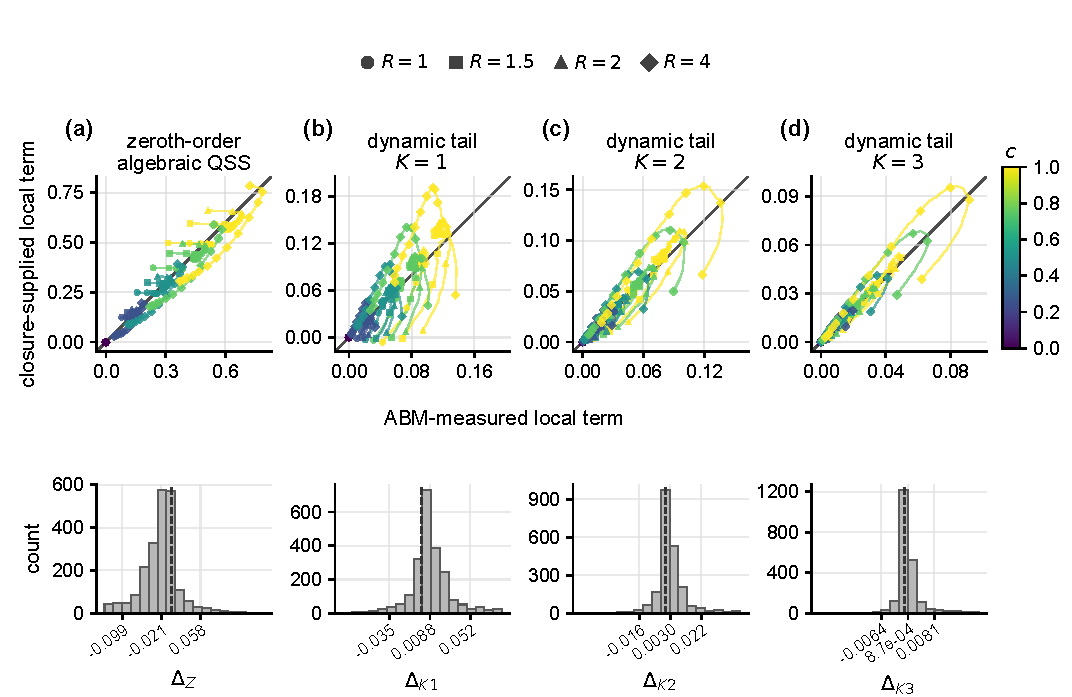
\includegraphics[width=\textwidth]{figures/supp_S6_closure_snapshot.pdf}
\caption{Local closure terms evaluated along ensemble-mean finite-population ABM trajectories. Each colored path comprises post-activation snapshots ($\tau\geq0.5$) obtained after averaging 120 independent realizations within each parameter cell; color denotes $c$ and marker shape denotes $R$. In the top row, the horizontal coordinate is the ABM-measured local term and the vertical coordinate is the closure-supplied local term; the diagonal denotes equality. (a) Zeroth-order algebraic QSS closure: $c\overline m_1^{\mathrm{ABM}}$ is compared with $c\widehat m_1^{(0)}(\overline R_S^{\mathrm{ABM}})$. (b--d) Dynamic tail closures $K=1,2,3$: $c[\overline m_1^{\mathrm{ABM}}\overline m_K^{\mathrm{ABM}} - \overline m_{K+1}^{\mathrm{ABM}}]$ is compared with $c[\overline m_1^{\mathrm{ABM}}\overline m_K^{\mathrm{ABM}} - \Phi_{K+1}^{\mathrm{tail}}(\overline R_S^{\mathrm{ABM}};\overline m_K^{\mathrm{ABM}})]$. All quantities in a snapshot are evaluated at the same ensemble-mean state, with $\overline R_S^{\mathrm{ABM}}=R\overline S^{\mathrm{ABM}}/S_0$. The bottom row shows descriptive snapshot distributions of the signed closure-supplied-minus-ABM-measured differences, labeled $\Delta_Z,\Delta_{K1},\Delta_{K2}$, and $\Delta_{K3}$. Histograms pool the displayed ensemble-mean snapshots with $c>0$; their three x-axis ticks are the mean minus two population standard deviations, the mean, and the mean plus two population standard deviations, rounded to two significant digits. Simulations use $S_0=8000$, $I_0=160$, $R\in\{1,1.5,2,4\}$, $c\in\{0,0.25,0.5,0.75,1\}$, and 151 observation times on $0\leq\tau\leq5$, with $(\gamma/\Gamma,\gamma_c/\Gamma,p_f)=(0,1,c)$. Normalized genealogical coordinates are averaged conditionally over realizations with positive infectious count.}
\label{fig:s6}
\end{figure}

\begin{figure}[H]
\centering
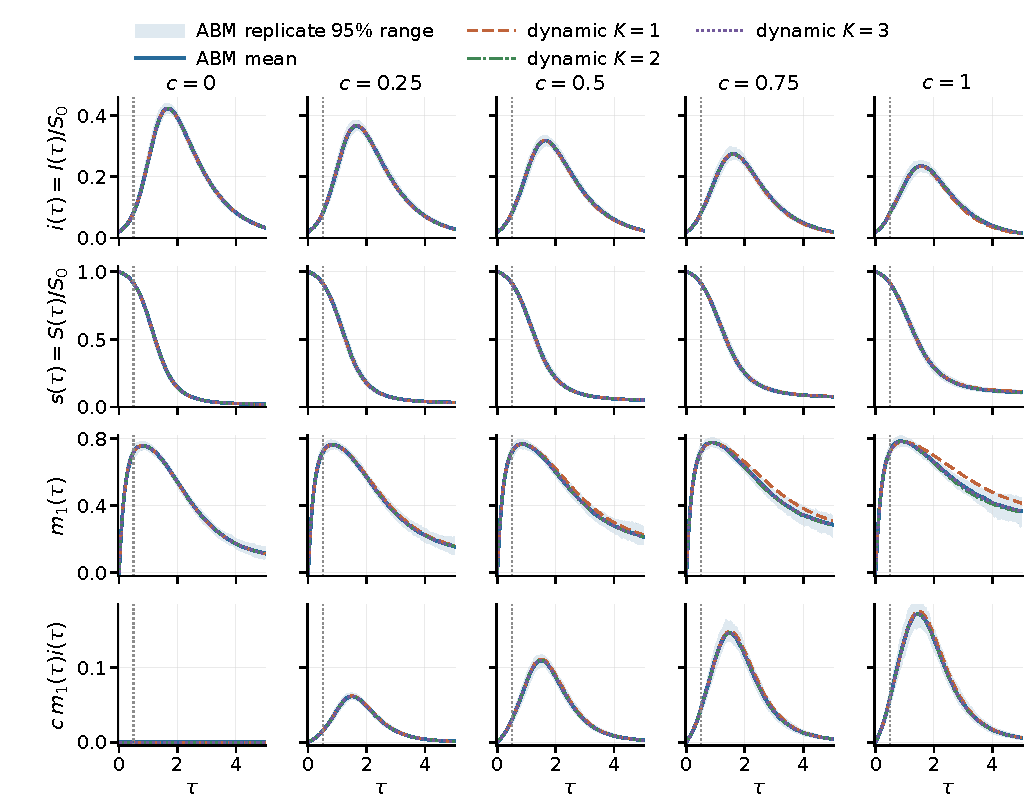
\includegraphics[width=\textwidth]{figures/supp_S7_depthK_trajectories.pdf}
\caption{Representative finite-pool trajectories for the depth-$K$ dynamic closures at $R=4$. Columns show $c=0,0.25,0.5,0.75$, and $1$; rows show $i=I/S_0$, $s=S/S_0$, $m_1=M_1/I$, and the normalized deterministic tracing flux $c\,m_1(\tau)i(\tau)$. Blue curves are the sample ensemble-mean ABM trajectory and pale bands are pointwise 2.5th--97.5th replicate percentiles across 120 independent realizations. Orange dashed, green dash-dotted, and purple dotted curves are the dynamic $K=1$, $2$, and $3$ closures. The vertical dotted line marks activation of forward tracing at $\tau=0.5$. Simulations use $S_0=8000$, $I_0=160$, and 151 observation times on $0\leq\tau\leq5$, with $(\gamma/\Gamma,\gamma_c/\Gamma,p_f)=(0,1,c)$. These are the same $R=4$ ABM replicates underlying the main-text closure-trajectory errors and algebraic-closure overlays.}
\label{fig:s7}
\end{figure}

\section*{S7 Reproducibility files}
\pdfbookmark[1]{S7 Reproducibility files}{s7}
Supplementary Material~2 provides the dimensional parameter table, the published error and convergence summaries, and the deterministic-reference and event-term diagnostics. Supplementary Material~3 provides the executable and audit code, the numerical and figure data, the figure-generation files, and the software requirements.

Within Supplementary Material~3, the material behind Sections~S2 and S3 comprises the complete Fig.~\ref{fig:S7-1} curve data, the maximum-error summary, the symbolic coefficient audit, the QSS solver diagnostics, and standalone generation scripts, stored under \texttt{data/}, \texttt{diagnostics/}, and \texttt{reproducibility/}; the symbolic audit independently verifies the displayed coefficients.

\section*{References}

The continued-fraction and special-function numerical procedures in Section~S2.2 use Gautschi (1967) and Olver et al. (2010).

\begin{list}{}{\setlength{\leftmargin}{1.2em}\setlength{\itemindent}{-1.2em}\setlength{\itemsep}{0.4em}}
\item Amos DE (1974) Computation of modified Bessel functions and their ratios. Math Comput 28:239--251. \url{https://doi.org/10.1090/S0025-5718-1974-0333287-7}
\item Gautschi W (1967) Computational aspects of three-term recurrence relations. SIAM Rev 9:24--82. \url{https://doi.org/10.1137/1009002}
\item Krantz SG, Parks HR (2002) The implicit function theorem: history, theory, and applications. Birkhäuser, Boston. \url{https://doi.org/10.1007/978-1-4612-0059-8}
\item Murdock JA (1999) Perturbations: theory and methods. Classics in Applied Mathematics, vol 27. SIAM, Philadelphia. \url{https://doi.org/10.1137/1.9781611971095}
\item Olver FWJ, Lozier DW, Boisvert RF, Clark CW (eds) (2010) NIST handbook of mathematical functions. Cambridge University Press, New York. \url{https://www.nist.gov/publications/nist-handbook-mathematical-functions}
\end{list}

\end{document}
